\pagenumbering{gobble} % suppress page numbering here
\newcommand{\NaturalElementTextFormat}[6]
{
	\begin{minipage}{2.21cm}
		\centering
		{\textbf{#1} \hfill {#2}\textit{{#3}}}%
		\\[0.1cm]
		{\Huge \textbf{{#5}}}
		\linebreak
		{#6}
		\linebreak
		{\small {#4}} 
	\end{minipage}
}

\newcommand{\KeyTextFormat}[6]
{
	\begin{minipage}{3.3cm}
		\centering
		{{\small \textbf{#1}} \hfill {#2} {#3}}%
		\\[0.7cm]
		
		{\Huge \textbf{{#5}}}
		\linebreak
		{#6}
		\linebreak
		{\small {#4}} 
		\linebreak
	\end{minipage}
}
\tikzstyle{SBlock} = [fill=white!10]
\tikzstyle{PBlock} = [fill=white!10]
\tikzstyle{DBlock} = [fill=white!10]
\tikzstyle{FBlock} = [fill=white!7]

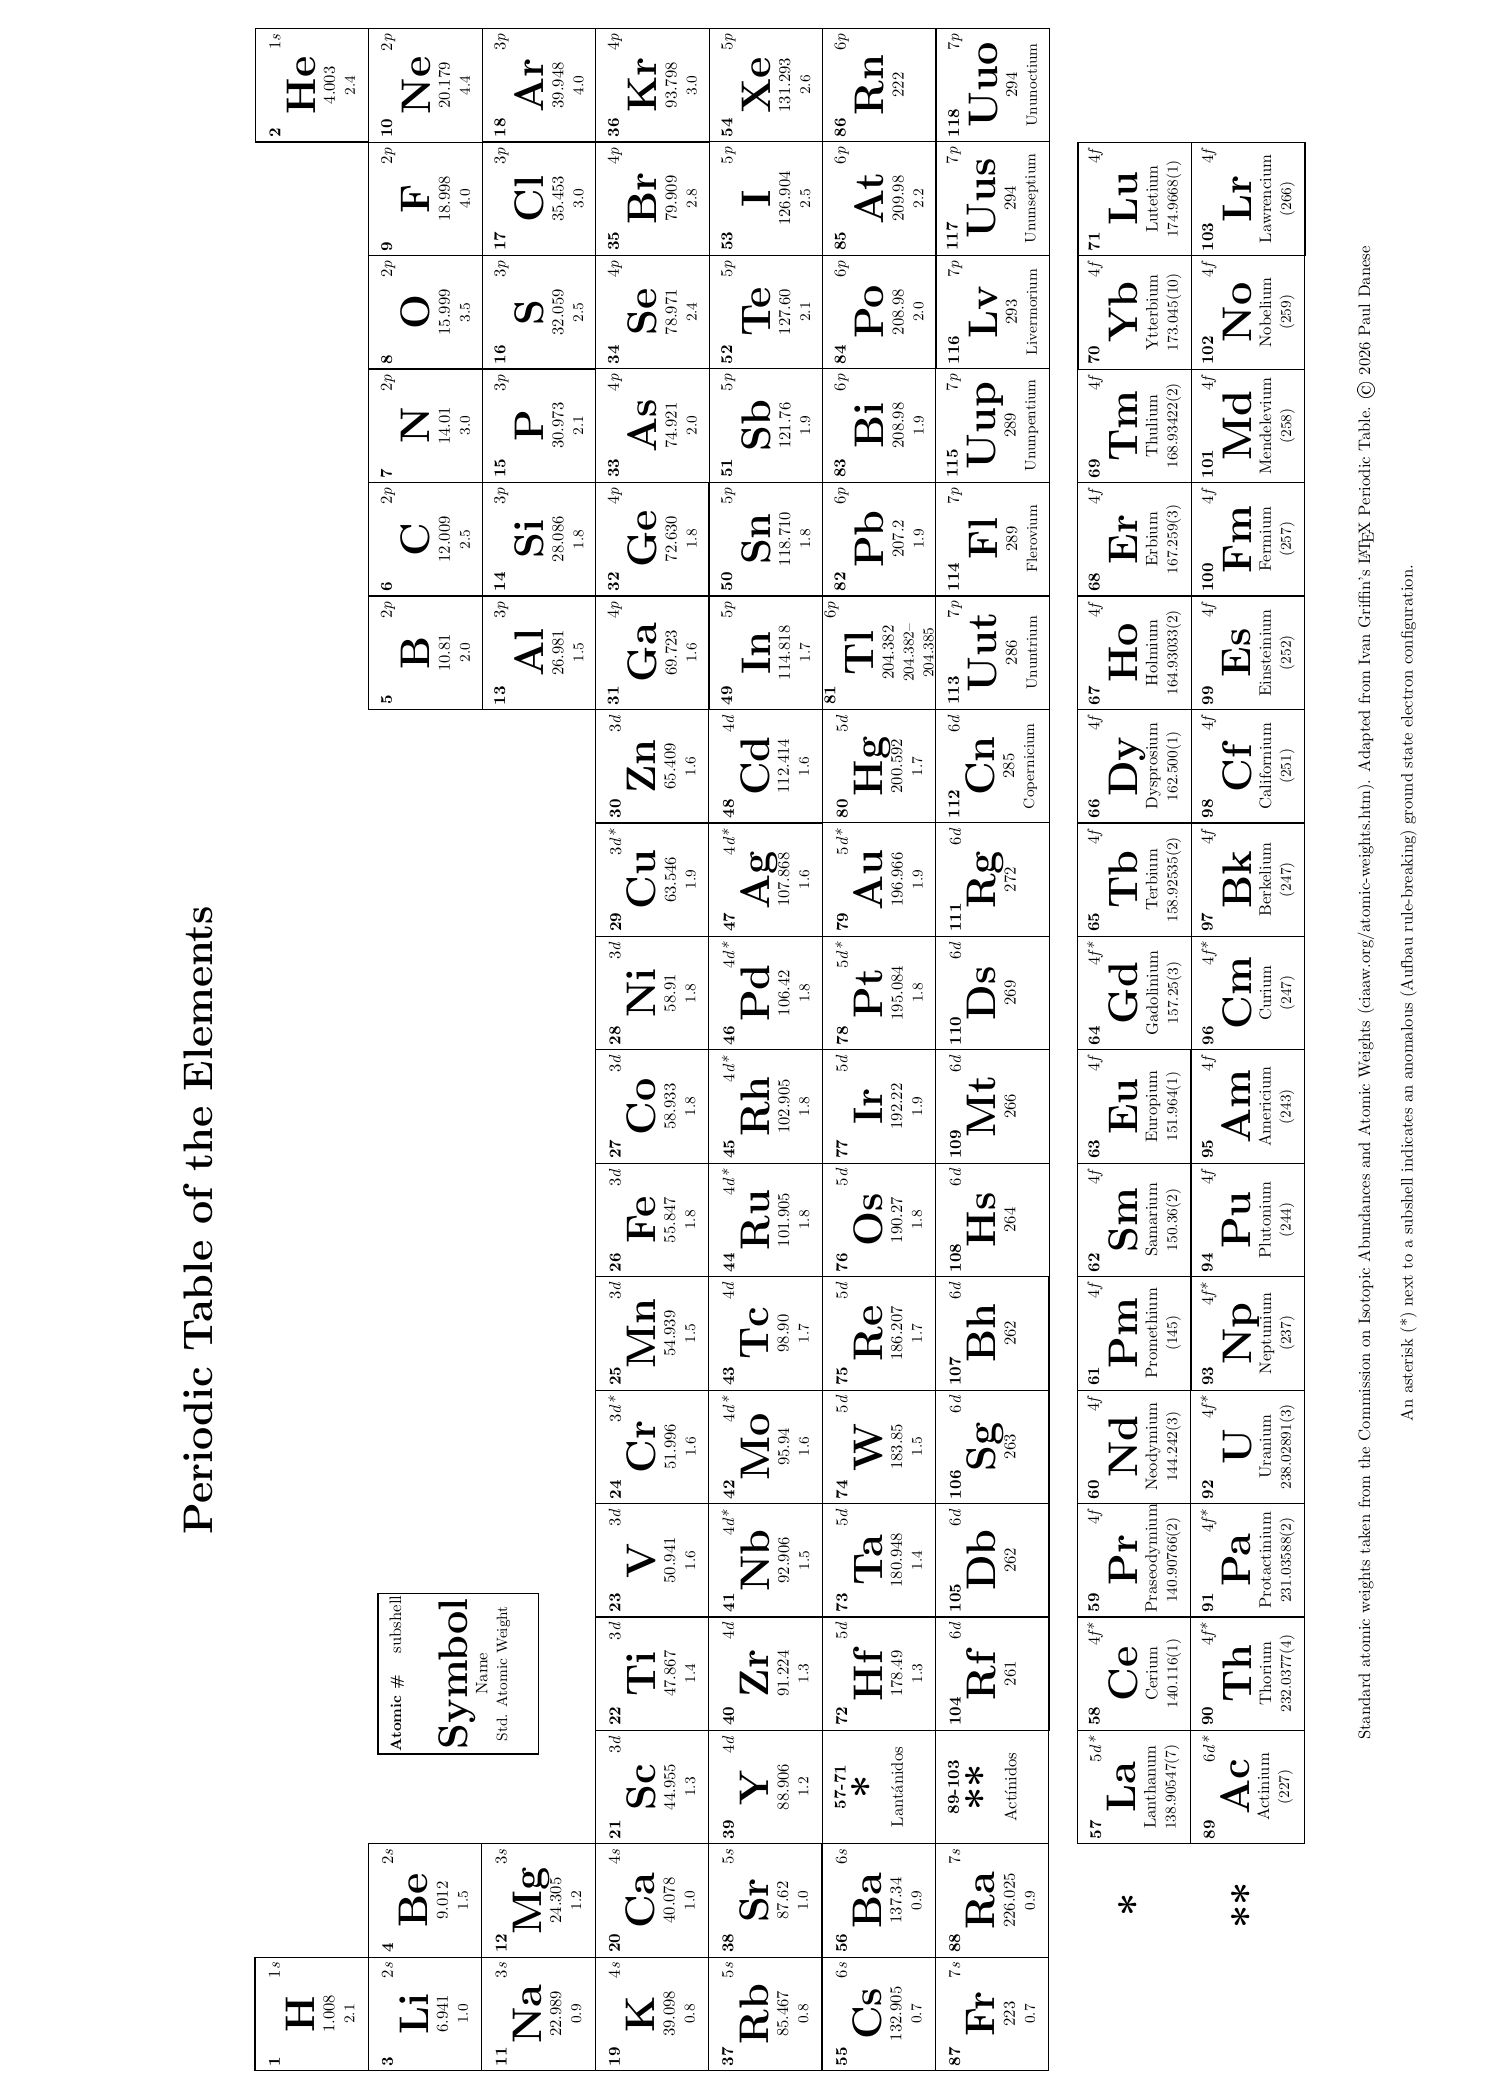
\begin{tikzpicture}[scale=0.6, transform shape, rotate=90]
	
	\tikzstyle{KeyBox} = [draw=black, minimum width=3.4cm, minimum height=3.4cm, node distance=3.4cm, inner sep=0pt]
	\tikzstyle{Element} = [draw=black, minimum width=2.4cm, minimum height=2.4cm, node distance=2.4cm, inner sep=0pt]
	\tikzstyle{Offsetter} = [draw=white, minimum width=2.4cm, minimum height=2.4cm, node distance=2.4cm, inner sep=0pt]
	\tikzstyle{TitleLabel} = [font={\Huge\bfseries}]
	\tikzstyle{DetailsLabel} = [minimum height = 2.5cm, node distance = 2.5cm, inner sep=0pt]
	
	%% Group 1 - IA
	\node[name=Blank1, Offsetter] {}; % this is just an invisible box that shoves the entire table downward to make it more centered
	\node[name=Blank2, below of=Blank1, Offsetter] {}; % see comment on invisible box above.
	\node[name=H,	below of=Blank2, SBlock, Element] {\NaturalElementTextFormat{1}{1}{s}{2.1}{H}{1.008}};
	\node[name=Li, 	below of=H, 	SBlock, Element] {\NaturalElementTextFormat{3}{2}{s}{1.0}{Li}{6.941}};
	\node[name=Na, 	below of=Li,	SBlock, Element] {\NaturalElementTextFormat{11}{3}{s}{0.9}{Na}{22.989}};
	\node[name=K, 	below of=Na,	SBlock, Element] {\NaturalElementTextFormat{19}{4}{s}{0.8}{K}{39.098}};
	\node[name=Rb, 	below of=K, 	SBlock, Element] {\NaturalElementTextFormat{37}{5}{s}{0.8}{Rb}{85.467}};
	\node[name=Cs, 	below of=Rb,	SBlock, Element] {\NaturalElementTextFormat{55}{6}{s}{0.7}{Cs}{132.905}};
	\node[name=Fr, 	below of=Cs,	SBlock, Element] {\NaturalElementTextFormat{87}{7}{s}{0.7}{Fr}{223}};
	
	%% Group 2 - IIA
	\node[name=Be, right of=Li, SBlock, Element] {\NaturalElementTextFormat{4}{2}{s}{1.5}{Be}{9.012}};
	\node[name=Mg, below of=Be, SBlock, Element] {\NaturalElementTextFormat{12}{3}{s}{1.2}{Mg}{24.305}};
	\node[name=Ca, below of=Mg, SBlock, Element] {\NaturalElementTextFormat{20}{4}{s}{1.0}{Ca}{40.078}};
	\node[name=Sr, below of=Ca, SBlock, Element] {\NaturalElementTextFormat{38}{5}{s}{1.0}{Sr}{87.62}};
	\node[name=Ba, below of=Sr, SBlock, Element] {\NaturalElementTextFormat{56}{6}{s}{0.9}{Ba}{137.34}};
	\node[name=Ra, below of=Ba, SBlock, Element] {\NaturalElementTextFormat{88}{7}{s}{0.9}{Ra}{226.025}};
	
	%% Group 3 - IIIB
	\node[name=Sc, 	right of=Ca, 	DBlock,  Element] {\NaturalElementTextFormat{21}{3}{d}{1.3}{Sc}{44.955}};
	\node[name=Y, 	below of=Sc, 	DBlock, Element] {\NaturalElementTextFormat{39}{4}{d}{1.2}{Y}{88.906}};
	\node[name=LaLu, 	below of=Y, 	Element] {\NaturalElementTextFormat{57-71}{}{}{}{*}{Lantánidos}};
	\node[name=AcLr, 	below of=LaLu, 	Element] {\NaturalElementTextFormat{89-103}{}{}{}{**}{Actínidos}};
	
	%% Group 4 - IVB
	\node[name=Ti, right of=Sc, DBlock, Element] {\NaturalElementTextFormat{22}{3}{d}{1.4}{Ti}{47.867}};
	\node[name=Zr, below of=Ti,DBlock,  Element] {\NaturalElementTextFormat{40}{4}{d}{1.3}{Zr}{91.224}};
	\node[name=Hf, below of=Zr,DBlock,  Element] {\NaturalElementTextFormat{72}{5}{d}{1.3}{Hf}{178.49}};
	\node[name=Rf, below of=Hf, DBlock, Element] {\NaturalElementTextFormat{104}{6}{d}{}{Rf}{261}};
	
	%% Group 5 - VB
	\node[name=V, right of=Ti, DBlock, Element] {\NaturalElementTextFormat{23}{3}{d}{1.6}{V}{50.941}};
	\node[name=Nb, below of=V, DBlock, Element] {\NaturalElementTextFormat{41}{4}{d*}{1.5}{Nb}{92.906}};
	\node[name=Ta, below of=Nb, DBlock, Element] {\NaturalElementTextFormat{73}{5}{d}{1.4}{Ta}{180.948}};
	\node[name=Db, below of=Ta, DBlock, Element] {\NaturalElementTextFormat{105}{6}{d}{}{Db}{262}};
	
	%% Group 6 - VIB
	\node[name=Cr, right of=V, DBlock, Element] {\NaturalElementTextFormat{24}{3}{d*}{1.6}{Cr}{51.996}};
	\node[name=Mo, below of=Cr,DBlock,  Element] {\NaturalElementTextFormat{42}{4}{d*}{1.6}{Mo}{95.94}};
	\node[name=W, below of=Mo,DBlock,  Element] {\NaturalElementTextFormat{74}{5}{d}{1.5}{W}{183.85}};
	\node[name=Sg, below of=W, DBlock, Element] {\NaturalElementTextFormat{106}{6}{d}{}{Sg}{263}};
	
	%% Group 7 - VIIB
	\node[name=Mn, right of=Cr, DBlock, Element] {\NaturalElementTextFormat{25}{3}{d}{1.5}{Mn}{54.939}};
	\node[name=Tc, below of=Mn, DBlock, Element] {\NaturalElementTextFormat{43}{4}{d}{1.7}{Tc}{98.90}};
	\node[name=Re, below of=Tc, DBlock, Element] {\NaturalElementTextFormat{75}{5}{d}{1.7}{Re}{186.207}};
	\node[name=Bh, below of=Re, DBlock, Element] {\NaturalElementTextFormat{107}{6}{d}{}{Bh}{262}};
	
	%% Group 8 - VIIIB
	\node[name=Fe, right of=Mn, DBlock, Element] {\NaturalElementTextFormat{26}{3}{d}{1.8}{Fe}{55.847}};
	\node[name=Ru, below of=Fe, DBlock, Element] {\NaturalElementTextFormat{44}{4}{d*}{1.8}{Ru}{101.905}};
	\node[name=Os, below of=Ru, DBlock, Element] {\NaturalElementTextFormat{76}{5}{d}{1.8}{Os}{190.27}};
	\node[name=Hs, below of=Os, DBlock, Element] {\NaturalElementTextFormat{108}{6}{d}{}{Hs}{264}};
	
	%% Group 9 - VIIIB
	\node[name=Co, right of=Fe,DBlock,  Element] {\NaturalElementTextFormat{27}{3}{d}{1.8}{Co}{58.933}};
	\node[name=Rh, below of=Co, DBlock, Element] {\NaturalElementTextFormat{45}{4}{d*}{1.8}{Rh}{102.905}};
	\node[name=Ir, below of=Rh, DBlock, Element] {\NaturalElementTextFormat{77}{5}{d}{1.9}{Ir}{192.22}};
	\node[name=Mt, below of=Ir, DBlock, Element] {\NaturalElementTextFormat{109}{6}{d}{}{Mt}{266}};
	
	%% Group 10 - VIIIB
	\node[name=Ni, right of=Co, DBlock, Element] {\NaturalElementTextFormat{28}{3}{d}{1.8}{Ni}{58.91}};
	\node[name=Pd, below of=Ni, DBlock, Element] {\NaturalElementTextFormat{46}{4}{d*}{1.8}{Pd}{106.42}};
	\node[name=Pt, below of=Pd, DBlock, Element] {\NaturalElementTextFormat{78}{5}{d*}{1.8}{Pt}{195.084}};
	\node[name=Ds, below of=Pt, DBlock, Element] {\NaturalElementTextFormat{110}{6}{d}{}{Ds}{269}};
	
	%% Group 11 - IB
	\node[name=Cu, right of=Ni, DBlock, Element] {\NaturalElementTextFormat{29}{3}{d*}{1.9}{Cu}{63.546}};
	\node[name=Ag, below of=Cu, DBlock, Element] {\NaturalElementTextFormat{47}{4}{d*}{1.6}{Ag}{107.868}};
	\node[name=Au, below of=Ag, DBlock, Element] {\NaturalElementTextFormat{79}{5}{d*}{1.9}{Au}{196.966}};
	\node[name=Rg, below of=Au,DBlock,  Element] {\NaturalElementTextFormat{111}{6}{d}{}{Rg}{272}};
	
	%% Group 12 - IIB
	\node[name=Zn, right of=Cu, DBlock, Element] {\NaturalElementTextFormat{30}{3}{d}{1.6}{Zn}{65.409}};
	\node[name=Cd, below of=Zn, DBlock, Element] {\NaturalElementTextFormat{48}{4}{d}{1.6}{Cd}{112.414}};
	\node[name=Hg, below of=Cd, DBlock, Element] {\NaturalElementTextFormat{80}{5}{d}{1.7}{Hg}{200.592}};
	\node[name=Uub, below of=Hg, DBlock, Element] {\NaturalElementTextFormat{112}{6}{d}{Copernicium}{Cn}{285}};
	
	%% Group 13 - IIIA
	\node[name=Ga, right of=Zn, PBlock,  Element] {\NaturalElementTextFormat{31}{4}{p}{1.6}{Ga}{69.723}};
	\node[name=Al, above of=Ga, PBlock,  Element] {\NaturalElementTextFormat{13}{3}{p}{1.5}{Al}{26.981}};
	\node[name=B, above of=Al, PBlock, Element] {\NaturalElementTextFormat{5}{2}{p}{2.0}{B}{10.81}};
	\node[name=In, below of=Ga, PBlock,  Element] {\NaturalElementTextFormat{49}{5}{p}{1.7}{In}{114.818}};
	\node[name=Tl, below of=In, PBlock,  Element] {\NaturalElementTextFormat{81}{6}{p}{204.382--204.385}{Tl}{204.382}};
	\node[name=Uut, below of=Tl, PBlock,  Element] {\NaturalElementTextFormat{113}{7}{p}{Ununtrium}{Uut}{286}};
	
	%% Group 14 - IVA
	\node[name=C, right of=B, PBlock, Element] {\NaturalElementTextFormat{6}{2}{p}{2.5}{C}{12.009}};
	\node[name=Si, below of=C,PBlock,  Element] {\NaturalElementTextFormat{14}{3}{p}{1.8}{Si}{28.086}};
	\node[name=Ge, below of=Si, PBlock, Element] {\NaturalElementTextFormat{32}{4}{p}{1.8}{Ge}{72.630}};
	\node[name=Sn, below of=Ge,PBlock,  Element] {\NaturalElementTextFormat{50}{5}{p}{1.8}{Sn}{118.710}};
	\node[name=Pb, below of=Sn, PBlock, Element] {\NaturalElementTextFormat{82}{6}{p}{1.9}{Pb}{207.2}};
	\node[name=Uuq, below of=Pb,PBlock,  Element] {\NaturalElementTextFormat{114}{7}{p}{Flerovium}{Fl}{289}};
	
	%% Group 15 - VA
	\node[name=N, right of=C, PBlock,  Element] {\NaturalElementTextFormat{7}{2}{p}{3.0}{N}{14.01}};
	\node[name=P, below of=N, PBlock,  Element] {\NaturalElementTextFormat{15}{3}{p}{2.1}{P}{30.973}};
	\node[name=As, below of=P,PBlock,   Element] {\NaturalElementTextFormat{33}{4}{p}{2.0}{As}{74.921}};
	\node[name=Sb, below of=As, PBlock,  Element] {\NaturalElementTextFormat{51}{5}{p}{1.9}{Sb}{121.76}};
	\node[name=Bi, below of=Sb, PBlock,  Element] {\NaturalElementTextFormat{83}{6}{p}{1.9}{Bi}{208.98}};
	\node[name=Uup, below of=Bi,PBlock,   Element] {\NaturalElementTextFormat{115}{7}{p}{Ununpentium}{Uup}{289}};
	
	%% Group 16 - VIA
	\node[name=O, right of=N,PBlock,   Element] {\NaturalElementTextFormat{8}{2}{p}{3.5}{O}{15.999}};
	\node[name=S, below of=O, PBlock,  Element] {\NaturalElementTextFormat{16}{3}{p}{2.5}{S}{32.059}};
	\node[name=Se, below of=S, PBlock,  Element] {\NaturalElementTextFormat{34}{4}{p}{2.4}{Se}{78.971}};
	\node[name=Te, below of=Se, PBlock,  Element] {\NaturalElementTextFormat{52}{5}{p}{2.1}{Te}{127.60}};
	\node[name=Po, below of=Te, PBlock,  Element] {\NaturalElementTextFormat{84}{6}{p}{2.0}{Po}{208.98}};
	\node[name=Uuh, below of=Po, PBlock,  Element] {\NaturalElementTextFormat{116}{7}{p}{Livermorium}{Lv}{293}};
	
	%% Group 17 - VIIA
	\node[name=F, right of=O, PBlock,  Element] {\NaturalElementTextFormat{9}{2}{p}{4.0}{F}{18.998}};
	\node[name=Cl, below of=F, PBlock,  Element] {\NaturalElementTextFormat{17}{3}{p}{3.0}{Cl}{35.453}};
	\node[name=Br, below of=Cl, PBlock,  Element] {\NaturalElementTextFormat{35}{4}{p}{2.8}{Br}{79.909}};
	\node[name=I, below of=Br, PBlock,  Element] {\NaturalElementTextFormat{53}{5}{p}{2.5}{I}{126.904}};
	\node[name=At, below of=I,PBlock,   Element] {\NaturalElementTextFormat{85}{6}{p}{2.2}{At}{209.98}};
	\node[name=Uus, below of=At, PBlock,  Element] {\NaturalElementTextFormat{117}{7}{p}{Ununseptium}{Uus}{294}}; 
	
	%% Group 18 - VIIIA
	\node[name=Ne, right of=F, PBlock,  Element] {\NaturalElementTextFormat{10}{2}{p}{4.4}{Ne}{20.179}};
	\node[name=He, above of=Ne,SBlock,  Element] {\NaturalElementTextFormat{2}{1}{s}{2.4}{He}{4.003}};
	\node[name=Ar, below of=Ne, PBlock,  Element] {\NaturalElementTextFormat{18}{3}{p}{4.0}{Ar}{39.948}};
	\node[name=Kr, below of=Ar, PBlock,  Element] {\NaturalElementTextFormat{36}{4}{p}{3.0}{Kr}{93.798}};
	\node[name=Xe, below of=Kr, PBlock,  Element] {\NaturalElementTextFormat{54}{5}{p}{2.6}{Xe}{131.293}};
	\node[name=Rn, below of=Xe, PBlock,  Element] {\NaturalElementTextFormat{86}{6}{p}{}{Rn}{222}};
	\node[name=Uuo, below of=Rn, PBlock,  Element] {\NaturalElementTextFormat{118}{7}{p}{Ununoctium}{Uuo}{294}}; 
	
	
	%% Lanthanide
	\node[name=La, below of=AcLr, DBlock, Element, yshift=-0.6cm] {\NaturalElementTextFormat{57}{5}{d*}{138.90547(7)}{La}{Lanthanum}};
	\node[name=Ce, right of=La, FBlock, Element] {\NaturalElementTextFormat{58}{4}{f*}{140.116(1)}{Ce}{Cerium}};
	\node[name=Pr, right of=Ce, FBlock, Element] {\NaturalElementTextFormat{59}{4}{f}{140.90766(2)}{Pr}{Praseodymium}};
	\node[name=Nd, right of=Pr, FBlock, Element] {\NaturalElementTextFormat{60}{4}{f}{144.242(3)}{Nd}{Neodymium}};
	\node[name=Pm, right of=Nd, FBlock, Element] {\NaturalElementTextFormat{61}{4}{f}{(145)}{Pm}{Promethium}};
	\node[name=Sm, right of=Pm, FBlock, Element] {\NaturalElementTextFormat{62}{4}{f}{150.36(2)}{Sm}{Samarium}};
	\node[name=Eu, right of=Sm, FBlock, Element] {\NaturalElementTextFormat{63}{4}{f}{151.964(1)}{Eu}{Europium}};
	\node[name=Gd, right of=Eu, FBlock, Element] {\NaturalElementTextFormat{64}{4}{f*}{157.25(3)}{Gd}{Gadolinium}};
	\node[name=Tb, right of=Gd, FBlock, Element] {\NaturalElementTextFormat{65}{4}{f}{158.92535(2)}{Tb}{Terbium}};
	\node[name=Dy, right of=Tb, FBlock, Element] {\NaturalElementTextFormat{66}{4}{f}{162.500(1)}{Dy}{Dysprosium}};
	\node[name=Ho, right of=Dy, FBlock, Element] {\NaturalElementTextFormat{67}{4}{f}{164.93033(2)}{Ho}{Holmium}};
	\node[name=Er, right of=Ho, FBlock, Element] {\NaturalElementTextFormat{68}{4}{f}{167.259(3)}{Er}{Erbium}};
	\node[name=Tm, right of=Er, FBlock, Element] {\NaturalElementTextFormat{69}{4}{f}{168.93422(2)}{Tm}{Thulium}};
	\node[name=Yb, right of=Tm, FBlock, Element] {\NaturalElementTextFormat{70}{4}{f}{173.045(10)}{Yb}{Ytterbium}};
	\node[name=Lu, right of=Yb, FBlock, Element] {\NaturalElementTextFormat{71}{4}{f}{174.9668(1)}{Lu}{Lutetium}};
	
	%% Actinide
	\node[name=Ac, below of=La, DBlock, Element] {\NaturalElementTextFormat{89}{6}{d*}{(227)}{Ac}{Actinium}};
	\node[name=Th, right of=Ac, FBlock, Element] {\NaturalElementTextFormat{90}{4}{f*}{232.0377(4)}{Th}{Thorium}};
	\node[name=Pa, right of=Th, FBlock, Element] {\NaturalElementTextFormat{91}{4}{f*}{231.03588(2)}{Pa}{Protactinium}};
	\node[name=U, right of=Pa, FBlock, Element] {\NaturalElementTextFormat{92}{4}{f*}{238.02891(3)}{U}{Uranium}};
	\node[name=Np, right of=U, FBlock, Element] {\NaturalElementTextFormat{93}{4}{f*}{(237)}{Np}{Neptunium}};
	\node[name=Pu, right of=Np, FBlock, Element] {\NaturalElementTextFormat{94}{4}{f}{(244)}{Pu}{Plutonium}};
	\node[name=Am, right of=Pu, FBlock, Element] {\NaturalElementTextFormat{95}{4}{f}{(243)}{Am}{Americium}};
	\node[name=Cm, right of=Am, FBlock, Element] {\NaturalElementTextFormat{96}{4}{f*}{(247)}{Cm}{Curium}};
	\node[name=Bk, right of=Cm, FBlock, Element] {\NaturalElementTextFormat{97}{4}{f}{(247)}{Bk}{Berkelium}};
	\node[name=Cf, right of=Bk, FBlock,  Element] {\NaturalElementTextFormat{98}{4}{f}{(251)}{Cf}{Californium}};
	\node[name=Es, right of=Cf, FBlock, Element] {\NaturalElementTextFormat{99}{4}{f}{(252)}{Es}{Einsteinium}};
	\node[name=Fm, right of=Es, FBlock, Element] {\NaturalElementTextFormat{100}{4}{f}{(257)}{Fm}{Fermium}};
	\node[name=Md, right of=Fm, FBlock, Element] {\NaturalElementTextFormat{101}{4}{f}{(258)}{Md}{Mendelevium}};
	\node[name=No, right of=Md, FBlock, Element] {\NaturalElementTextFormat{102}{4}{f}{(259)}{No}{Nobelium}};
	\node[name=Lr, right of=No, FBlock, Element] {\NaturalElementTextFormat{103}{4}{f}{(266)}{Lr}{Lawrencium}};
	\node[name=Star, left of=La, Offsetter, xshift=-0.1cm] {{\textbf{\Huge *}}};
	\node[name=DoubleStar, below of=Star, Offsetter] {{\textbf{\Huge **}}};
	
	\node[name=Key, above of=Ti, KeyBox, yshift=0.7cm] {\KeyTextFormat{Atomic \#}{subshell}{}{Std. Atomic Weight}{Symbol}{Name}};
	
	\node at (Blank2.west -| Fe.north) [name=diagramTitle, TitleLabel]
	{Periodic Table of the Elements};
	
	\node[below of=Cm, name=details, DetailsLabel]{Standard atomic weights taken from the Commission on Isotopic Abundances and Atomic Weights (ciaaw.org/atomic-weights.htm). Adapted from Ivan Griffin's \LaTeX\space Periodic Table. \textcopyright\space \the\year\space Paul Danese};
	\node[below of=details, DetailsLabel, yshift=1.6cm]{An asterisk (*) next to a subshell indicates an anomalous (Aufbau rule-breaking) ground state electron configuration.};
\end{tikzpicture}